\documentclass{beamer}
\usepackage{amsmath}
\usepackage[english]{babel} %set language; note: after changing this, you need to delete all auxiliary files to recompile
\usepackage[utf8]{inputenc} %define file encoding; latin1 is the other often used option
\usepackage{csquotes} % provides context sensitive quotation facilities
\usepackage{graphicx} %allows for inserting figures
\usepackage{booktabs} % for table formatting without vertical lines
\usepackage{textcomp} % allow for example using the Euro sign with \texteuro
\usepackage{stackengine}
\usepackage{wasysym}
\usepackage{tikzsymbols}
\usepackage{textcomp}
\newcommand{\bubblethis}[2]{
        \tikz[remember picture,baseline]{\node[anchor=base,inner sep=0,outer sep=0]%
        (#1) {\underline{#1}};\node[overlay,cloud callout,callout relative pointer={(0.2cm,-0.7cm)},%
        aspect=2.5,fill=yellow!90] at ($(#1.north)+(-0.5cm,1.6cm)$) {#2};}%
    }%
\tikzset{face/.style={shape=circle,minimum size=4ex,shading=radial,outer sep=0pt,
        inner color=white!50!yellow,outer color= yellow!70!orange}}
%% Some commands to make the code easier
\newcommand{\emoticon}[1][]{%
  \node[face,#1] (emoticon) {};
  %% The eyes are fixed.
  \draw[fill=white] (-1ex,0ex) ..controls (-0.5ex,0.2ex)and(0.5ex,0.2ex)..
        (1ex,0.0ex) ..controls ( 1.5ex,1.5ex)and( 0.2ex,1.7ex)..
        (0ex,0.4ex) ..controls (-0.2ex,1.7ex)and(-1.5ex,1.5ex)..
        (-1ex,0ex)--cycle;}
\newcommand{\pupils}{
  %% standard pupils
  \fill[shift={(0.5ex,0.5ex)},rotate=80] 
       (0,0) ellipse (0.3ex and 0.15ex);
  \fill[shift={(-0.5ex,0.5ex)},rotate=100] 
       (0,0) ellipse (0.3ex and 0.15ex);}

\newcommand{\emoticonname}[1]{
  \node[below=1ex of emoticon,font=\footnotesize,
        minimum width=4cm]{#1};}
\usepackage{scalerel}
\usetikzlibrary{positioning}
\usepackage{xcolor,amssymb}
\newcommand\dangersignb[1][2ex]{%
  \scaleto{\stackengine{0.3pt}{\scalebox{1.1}[.9]{%
  \color{red}$\blacktriangle$}}{\tiny\bfseries !}{O}{c}{F}{F}{L}}{#1}%
}
\newcommand\dangersignw[1][2ex]{%
  \scaleto{\stackengine{0.3pt}{\scalebox{1.1}[.9]{%
  \color{red}$\blacktriangle$}}{\color{white}\tiny\bfseries !}{O}{c}{F}{F}{L}}{#1}%
}
\usepackage{fontawesome} % Social Icons
\usepackage{epstopdf} % allow embedding eps-figures
\usepackage{tikz} % allows drawing figures
\usepackage{amsmath,amssymb,amsthm} %advanced math facilities
\usepackage{lmodern} %uses font that support italic and bold at the same time
\usepackage{hyperref}
\usepackage{tikz}
\hypersetup{
    colorlinks=true,
    linkcolor=blue,
    filecolor=magenta,      
    urlcolor=blue,
}
\usepackage{tcolorbox}
%add citation management using BibLaTeX
\usepackage[citestyle=authoryear-comp, %define style for citations
    bibstyle=authoryear-comp, %define style for bibliography
    maxbibnames=10, %maximum number of authors displayed in bibliography
    minbibnames=1, %minimum number of authors displayed in bibliography
    maxcitenames=3, %maximum number of authors displayed in citations before using et al.
    minnames=1, %maximum number of authors displayed in citations before using et al.
    datezeros=false, % do not print dates with leading zeros
    date=long, %use long formats for dates
    isbn=false,% show no ISBNs in bibliography (applies only if not a mandatory field)
    url=false,% show no urls in bibliography (applies only if not a mandatory field)
    doi=false, % show no dois in bibliography (applies only if not a mandatory field)
    eprint=false, %show no eprint-field in bibliography (applies only if not a mandatory field)
    backend=biber %use biber as the backend; backend=bibtex is less powerful, but easier to install
    ]{biblatex}
\addbibresource{../mybibfile.bib} %define bib-file located one folder higher


\usefonttheme[onlymath]{serif} %set math font to serif ones

\definecolor{beamerblue}{rgb}{0.2,0.2,0.7} %define beamerblue color for later use

%%% defines highlight command to set text blue
\newcommand{\highlight}[1]{{\color{blue}{#1}}}


%%%%%%% commands defining backup slides so that frame numbering is correct

\newcommand{\backupbegin}{
   \newcounter{framenumberappendix}
   \setcounter{framenumberappendix}{\value{framenumber}}
}
\newcommand{\backupend}{
   \addtocounter{framenumberappendix}{-\value{framenumber}}
   \addtocounter{framenumber}{\value{framenumberappendix}}
}

%%%% end of defining backup slides

%Specify figure caption, see also http://tex.stackexchange.com/questions/155738/caption-package-not-working-with-beamer
\setbeamertemplate{caption}{\insertcaption} %redefines caption to remove label "Figure".
%\setbeamerfont{caption}{size=\scriptsize,shape=\itshape,series=\bfseries} %sets figure  caption bold and italic and makes it smaller


\usetheme{Boadilla}

%set options of hyperref package
\hypersetup{
    bookmarksnumbered=true, %put section numbers in bookmarks
    naturalnames=true, %use LATEX-computed names for links
    citebordercolor={1 1 1}, %color of border around cites, here: white, i.e. invisible
    linkbordercolor={1 1 1}, %color of border around links, here: white, i.e. invisible
    colorlinks=true, %color links
    anchorcolor=black, %set color of anchors
    linkcolor=beamerblue, %set link color to beamer blue
    citecolor=blue, %set cite color to beamer blue
    pdfpagemode=UseThumbs, %set default mode of PDF display
    breaklinks=true, %break long links
    pdfstartpage=1 %start at first page
    }


% --------------------
% Overall information
% --------------------
% --------------------
% Overall information
% --------------------
\title[Economía I]{Economía I \vspace{4mm}
\\ Magistral 21: Mercado de trabajo}
\date{}
\author[Ertola Navajas y Fariña]{Ertola Navajas y Fariña}
\vspace{0.4cm}
\institute[]{Universidad de San Andrés} 


\begin{document}

\begin{frame}
\titlepage
\centering
Magistral 21


\includegraphics[scale=0.2]{Slides Principios de Economia/Figures/logoUDESA.jpg} 
\end{frame}


\begin{frame}{Mercado de trabajo: definiciones}
\begin{itemize}
    \item ¿Quiénes ofrecen trabajo?
    \vspace{2mm}
    \item ¿Quiénes demandan trabajo?
\end{itemize} 
\end{frame}


\begin{frame}{Mercado de trabajo: demanda de trabajo}
\begin{itemize}
\item Depende de los precios y de la productividad 
\end{itemize}
\begin{center}
\begin{figure}[H]
\renewcommand{\figurename}{Figure}
\begin{center}
\begin{tikzpicture}[scale=0.6]
\draw[very thick,<->] (0,11) node[left]{$W$}--(0,0)--(11,0) node[below]{$T$};
\draw[thin] (1,9).. controls (2,3) and (4, 2.5) .. (9, 1.5);
\node [] at (9.5,2.5) {\footnotesize Demanda};
\node [] at (9.5,2) {\footnotesize de trabajo};
\end{tikzpicture}
\end{center}
\end{figure}
\end{center} 
\end{frame}


\begin{frame}{Mercado de trabajo: oferta de trabajo}

\begin{itemize}
    \item ¿ Cómo responde la oferta de trabajo ante un cambio en los salarios?
    \vspace{2mm}
    \begin{itemize}
    \item Shock temporario $\Rightarrow$ la oferta de trabajo aumenta \vspace{1mm}
    \item Shock permanente $\Rightarrow$ la oferta de trabajo no se modifica (mucho) \vspace{1mm}
   \item Un ejemplo que ilustra esto último: desde la época medieval hemos trabajado aprox unas 8 horas por día
    \end{itemize}
\end{itemize}
\end{frame}

\begin{frame}{Mercado de trabajo: oferta de trabajo}
\begin{figure}[H]
\renewcommand{\figurename}{Figure}
\begin{center}
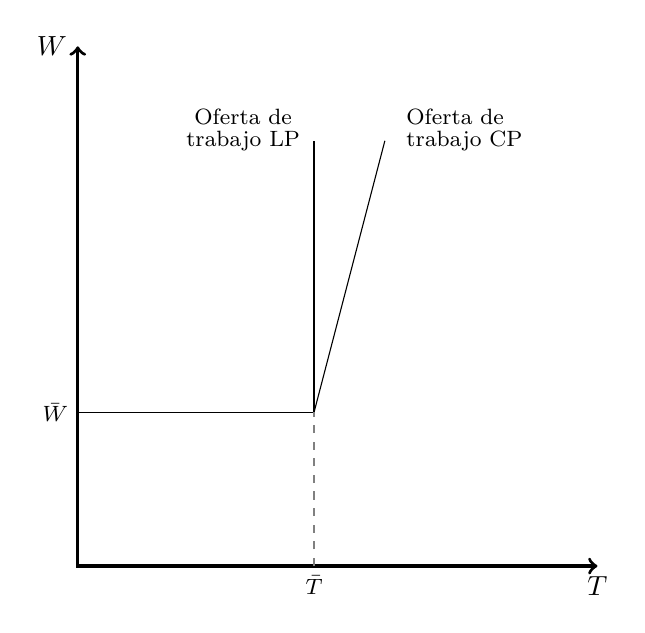
\begin{tikzpicture}[scale=0.6]
\draw[very thick,<->] (0,11) node[left]{$W$}--(0,0)--(11,0) node[below]{$T$};
\draw[thin](5,3.25)--(5,9);
\node [] at (3.5,9.5) {\footnotesize Oferta de};
\node [] at (3.5,9) {\footnotesize  trabajo LP};
\draw[thin](5,3.25)--(6.5,9);
\node [right] at (6.75,9.5) {\footnotesize Oferta de};
\node [right] at (6.75,9) {\footnotesize  trabajo CP};
\draw[thin](5,3.25)--(0,3.25);
\node [left] at (0,3.25) {\footnotesize  $\bar{W}$};
\draw[thick,gray,dashed](5,0)--(5,3.25);
\node[below] at (5,0) {\footnotesize $\bar{T}$};
\end{tikzpicture}
\end{center}
\end{figure}
\end{frame}

\begin{frame}{Mercado de trabajo: el equilibrio}
\begin{itemize}
    \item Si el salario está por encima de su valor de equilibrio (salario real*) habrá desempleo
\end{itemize}

\begin{center}
\begin{figure}[H]
\renewcommand{\figurename}{Figure}
\begin{center}
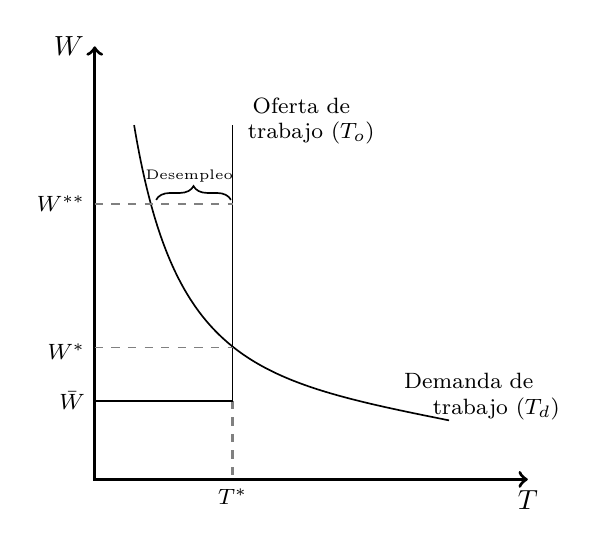
\begin{tikzpicture}[scale=0.5]
\draw[very thick,<->] (0,11) node[left]{$W$}--(0,0)--(11,0) node[below]{$T$};
\draw[semithick] (1,9).. controls (2,3) and (4, 2.5) .. (9, 1.5);
\node [] at (9.5,2.5) {\footnotesize Demanda de};
\node [] at (10.2,1.8) {\footnotesize trabajo ($T_d$)};
\draw[semithick](3.5,2)--(3.5,9);
\draw[thick, dashed, gray] (3.5,2)--(3.5,0);
\node [] at (5.25,9.5) {\footnotesize Oferta de};
\node [] at (5.5,8.8) {\footnotesize  trabajo ($T_o$)};
\node [below] at (3.5,0) {\footnotesize  $T^*$};
\node [left] at (0,3.25) {\footnotesize  $W^*$};
\draw[semithick, dashed,gray] (0,3.35)--(3.5,3.35);
\node [left] at (0,7) {\footnotesize  $W^{**}$};
\draw[semithick, dashed,gray] (0,7)--(3.5,7);
\draw (2.4,7.7) node[]{\tiny Desempleo};
\draw [semithick,decorate,decoration={brace,amplitude=5pt},xshift=-4pt,yshift=0pt](1.7,7.1) -- (3.6,7.1);
\node [left] at (0,2) {\footnotesize  $\bar{W}$}  ;
\draw[semithick] (0,2)--(3.5,2);
\end{tikzpicture}
\end{center}
\end{figure}
\end{center}  
\end{frame}


\begin{frame}{La visión de los Clásicos}
\begin{itemize}
    \item Según esta visión el mercado de trabajo siempre está en equilibrio:
    \vspace{2mm}
    \begin{itemize}
    \scriptsize\item Es decir que el salario real* es el de equilibrio
    \scriptsize\item De esta manera, el nivel de actividad es siempre el de pleno empleo
    \scriptsize \item Y la oferta agregada es vertical
    \end{itemize}
\end{itemize}

\begin{figure}[H]
\renewcommand{\figurename}{Figure}
\begin{center}
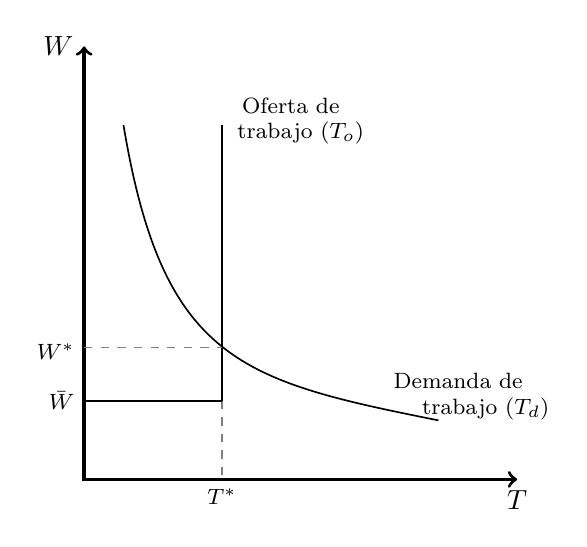
\begin{tikzpicture}[scale=0.5]
\draw[very thick,<->] (0,11) node[left]{$W$}--(0,0)--(11,0) node[below]{$T$};
\draw[semithick] (1,9).. controls (2,3) and (4, 2.5) .. (9, 1.5);
\node [] at (9.5,2.5) {\footnotesize Demanda de};
\node [] at (10.2,1.8) {\footnotesize trabajo ($T_d$)};
\draw[semithick](3.5,2)--(3.5,9);
\draw[thick, dashed, gray] (3.5,2)--(3.5,0);
\node [] at (5.25,9.5) {\footnotesize Oferta de};
\node [] at (5.5,8.8) {\footnotesize  trabajo ($T_o$)};
\node [below] at (3.5,0) {\footnotesize  $T^*$};
\node [left] at (0,3.25) {\footnotesize  $W^*$};
\draw[semithick, dashed,gray] (0,3.35)--(3.5,3.35);
%\draw[semithick, dashed,gray] (0,7)--(3.5,7);
%\draw [semithick,decorate,decoration={brace,amplitude=5pt},xshift=-4pt,yshift=0pt](1.7,7.1) -- (3.6,7.1);
\node [left] at (0,2) {\footnotesize  $\bar{W}$}  ;
\draw[semithick] (0,2)--(3.5,2);
\end{tikzpicture}
\end{center}
\end{figure}

\end{frame}


\begin{frame}{¿Y el desempleo?}
    \centering
\includegraphics[width=5cm]{Slides Principios de Economia/Figures/P29b.png}\
\begin{itemize}
\item Desempleo Friccional
\item Salarios de reserva altos
\item Problemas de medición
\end{itemize}
\end{frame}


\begin{frame}{La visión Keynesiana}
\begin{itemize}
    \footnotesize\item El mercado de trabajo \textbf{no siempre} está en equilibrio:
    \vspace{2mm}
    \begin{itemize}
    \scriptsize\item ¿Por qué puede el salario real permanecer fuera del equilibrio?
    \begin{itemize}
        \scriptsize\item Rigideces nominales
        \scriptsize\item Sindicatos
        \scriptsize\item Contratos de largo plazo
        \scriptsize\item Salarios de eficiencia
       \end{itemize}
       \item Un aumento en la demanda por trabajo aumenta el nivel de actividad con un efecto reducido en salarios y precios.
    \end{itemize}
\end{itemize}


\begin{center}
\begin{figure}[H]
\renewcommand{\figurename}{Figure}
\begin{center}
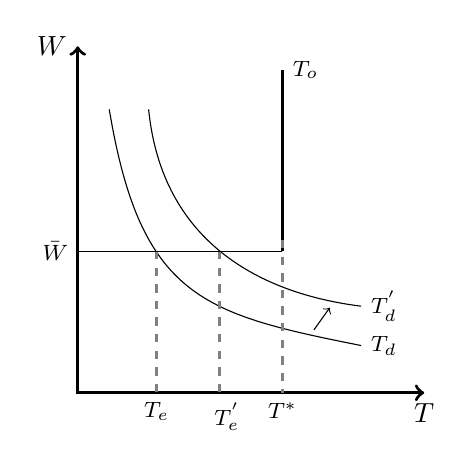
\begin{tikzpicture}[scale=0.4]
\draw[very thick,<->] (0,11) node[left]{$W$}--(0,0)--(11,0) node[below]{$T$};
\draw[thin] (1,9).. controls (2,3) and (4, 2.5) .. (9, 1.5) node [right]{\footnotesize $T_d$};
\draw[thin] (2.25,9).. controls (2.75,4) and (7, 3) .. (9, 2.75) node [right]{\footnotesize $T_d^{'}$};
\draw[thick,gray, dashed](2.5, 4.5)--(2.5, 0);
\node[below] at (2.5,0) {\footnotesize $T_e$};
\draw[thick,gray, dashed](4.5, 4.5)--(4.5, 0);
\node[below] at (4.75,0) {\footnotesize $T_e^{'}$};
\draw[thick](6.5, 4.5)--(6.5, 10.25) node [right]{\footnotesize $T_o$};
\draw[thick, gray, dashed] (6.5,4.85)--(6.5,0);
\node[below] at (6.5,0) {\footnotesize $T^*$};
\draw[thin](6.5, 4.5)--(0,4.5);
\node[left] at (0,4.5){\footnotesize $\Bar{W}$};
\draw[thin, ->] (7.5,2)--(8,2.7);
\end{tikzpicture}
\end{center}
\end{figure}
\end{center}  
\end{frame}


\begin{frame}{Motivos de desempleo}

\begin{itemize}
    \item Salario de  eficiencia
    \item Seguro de desempleo
    \item Sindicados
    \item Rigidices del mercado - Acuerdos nacionales o por empresa    
\end{itemize}

\end{frame}

\begin{frame}{Repasemos.....}

    \begin{itemize}
        \item Para los \textbf{Clásicos} es la capacidad productiva \faCogs:
            \begin{center}
            \begin{tcolorbox}[width=2in,
                  interior hidden,
                  boxsep=0pt,
                  left=0pt,
                  right=0pt,
                  top=2pt,
                  ]%%
                    $$ \bar{Y}=f(K, L) $$
             \end{tcolorbox}
             \end{center}
             
            \begin{itemize}
            \item El mercado de trabajo determina el empleo
            \item Se produce el PBI "potencial"
              \item "Ley de Say" (la oferta encuentra su demanda)
            \end{itemize}
        
        \item Para los \textbf{Keynesianos} es la demanda \faShoppingBasket:
            
            \begin{center}
            \begin{tcolorbox}[width=2in,
                  interior hidden,
                  boxsep=0pt,
                  left=0pt,
                  right=0pt,
                  top=2pt,
                  ]%%
                    $$ Y = C + I + G $$
             \end{tcolorbox}
             \end{center}
             
            \begin{itemize}
            \item El producto lo determina la demanda agregada
            \item ...si la demanda se ubica por debajo de la capacidad productiva de una economía
            \end{itemize}
    \end{itemize}

\end{frame}


\begin{frame}{El enfoque Clásico y Keynesiano: Demanda Agregada}

\centering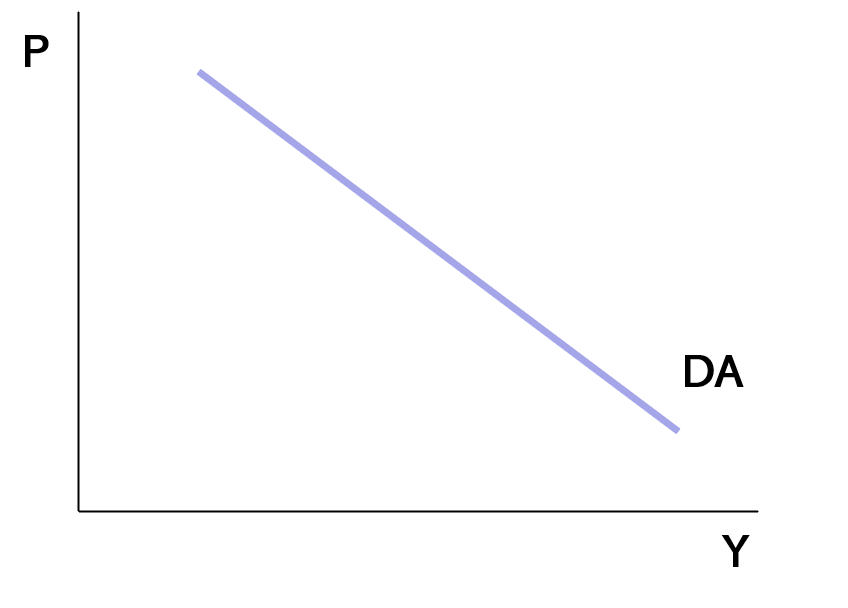
\includegraphics[width=6cm]{Slides Principios de Economia/Figures/P20.png}\

    \begin{itemize}
        \item La forma de esta curva determina como C (consumo) e I (inversión) reaccionan frente al nivel de P (precios)
        \item El consumo y la inversión caen debido al incremento en los precios:
            \begin{itemize}
                \item Efecto riqueza
                \item Efecto tasa de interés: un aumento de P sin cambiar M lleva a tasas de interés más altas que hacen caer C e I.
            \end{itemize}
    \end{itemize}

\end{frame}


\begin{frame}{Oferta Agregada y el mercado de trabajo}


\end{frame}


\begin{frame}{El enfoque Clásico y Keynesiano: Oferta Agregada}

\begin{itemize}
        \footnotesize\item La curva OA relaciona P (precios) con Y (producto).
        \footnotesize\item La forma de esta curva determina el mercado de trabajo.
\end{itemize}
\vspace{3mm}
\centering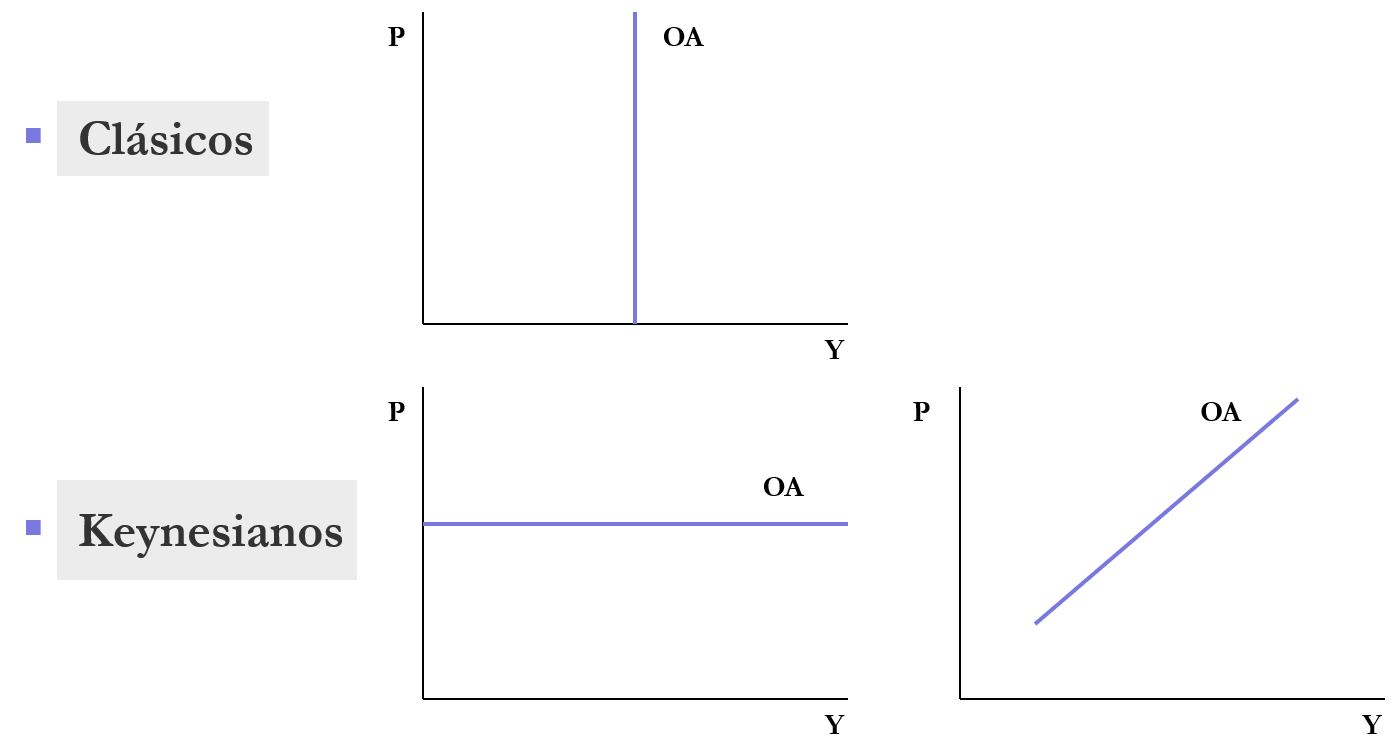
\includegraphics[width=10.5cm]{Slides Principios de Economia/Figures/P19.png}\

\end{frame}



\begin{frame}{Shocks a la Demanda Agregada}
    
\centering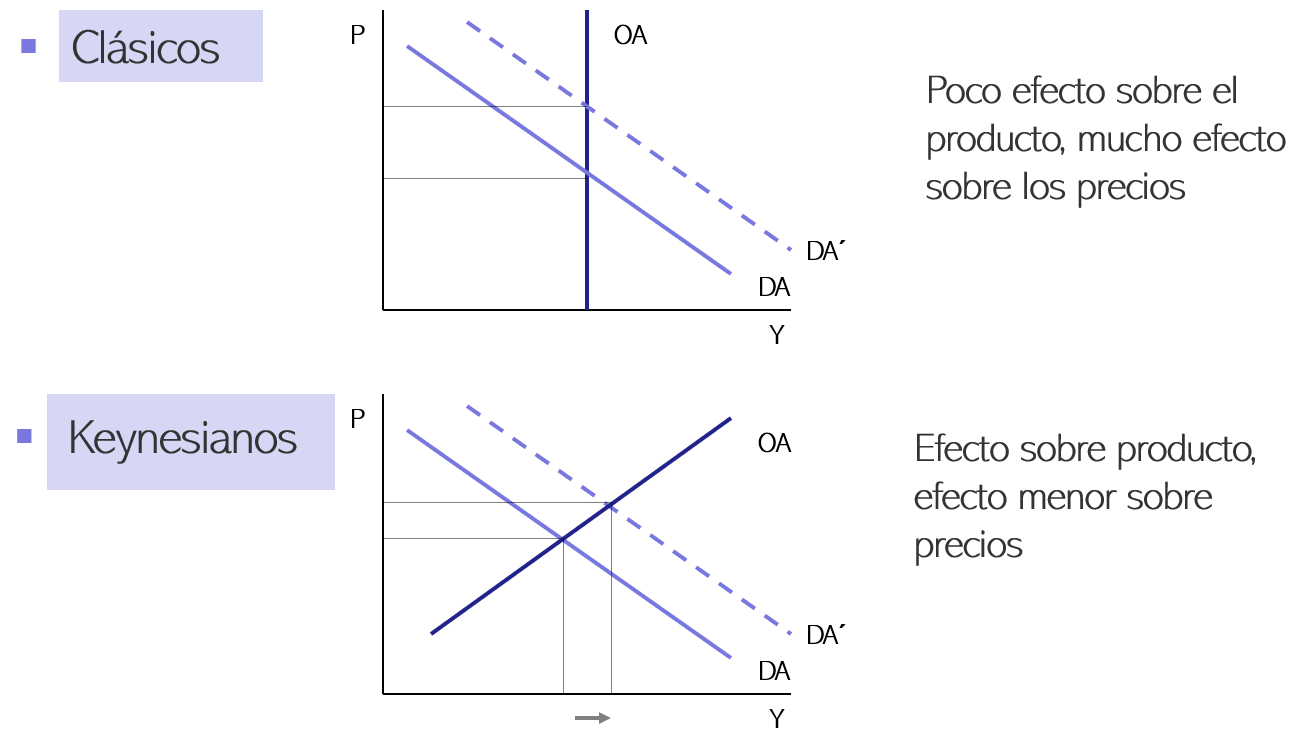
\includegraphics[width=11cm]{Slides Principios de Economia/Figures/P21.png}\
    
\end{frame}


\begin{frame}{Shocks a la Oferta Agregada}

Los shocks de oferta negativos  producen un fenómeno que se conoce como estanflación

\begin{figure} [H]
\centering
\begin{minipage}{.5\textwidth}
  \centering
  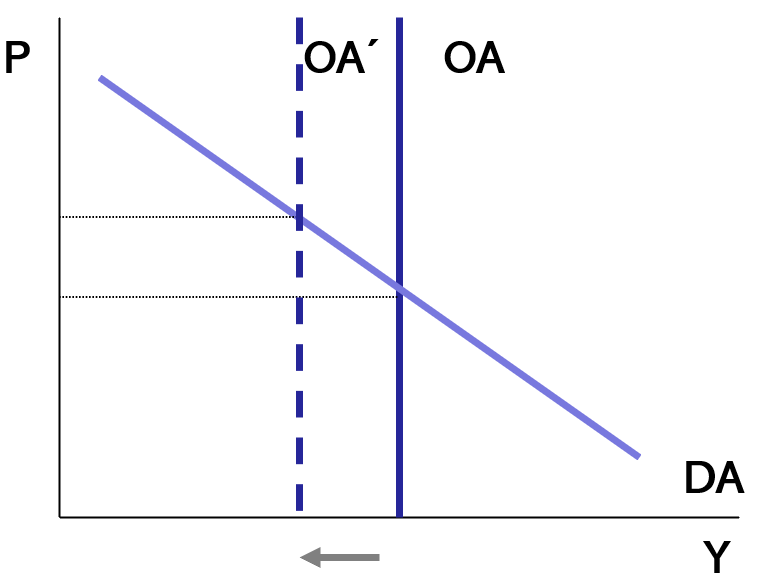
\includegraphics[width=0.9\textwidth]{Slides Principios de Economia/Figures/P22_1.png}
  \caption{\textbf{Clásicos}}
  \label{a}
\end{minipage}%
\begin{minipage}{.5\textwidth}
  \centering
  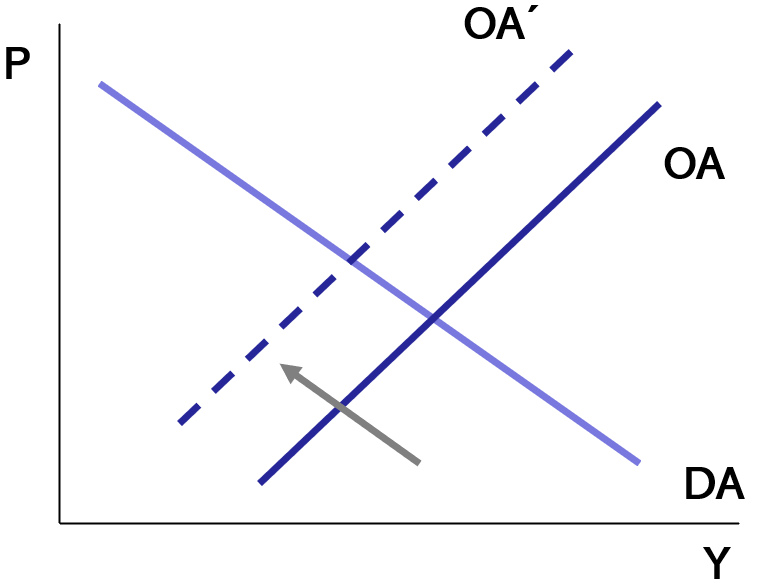
\includegraphics[width=0.9\textwidth]{Slides Principios de Economia/Figures/P22_2.png}
  \caption{\textbf{Keynesianos}}
  \label{b}
\end{minipage}
\\
\end{figure}

\end{frame}

\begin{frame}{Motivos de desempleo}

\begin{itemize}
    \item Salario de  eficiencia
    \item Seguro de desempleo
    \item Sindicados
    \item Rigidices del mercado - Acuerdos nacionales o por empresa    
\end{itemize}

\end{frame}



\begin{frame}{¿Qué es el desempleo y cómo se mide?}
\begin{itemize}
    \item Desempleo involuntario: es el desempleo de la gente que busca pero no encuentra empleo
    \item Fuerza laboral: PEA (Población Económicamente Activa)
        \begin{itemize}
            \item Empleados
            \item Desempleados
        \end{itemize}
\end{itemize}
\vspace{3mm}
\centering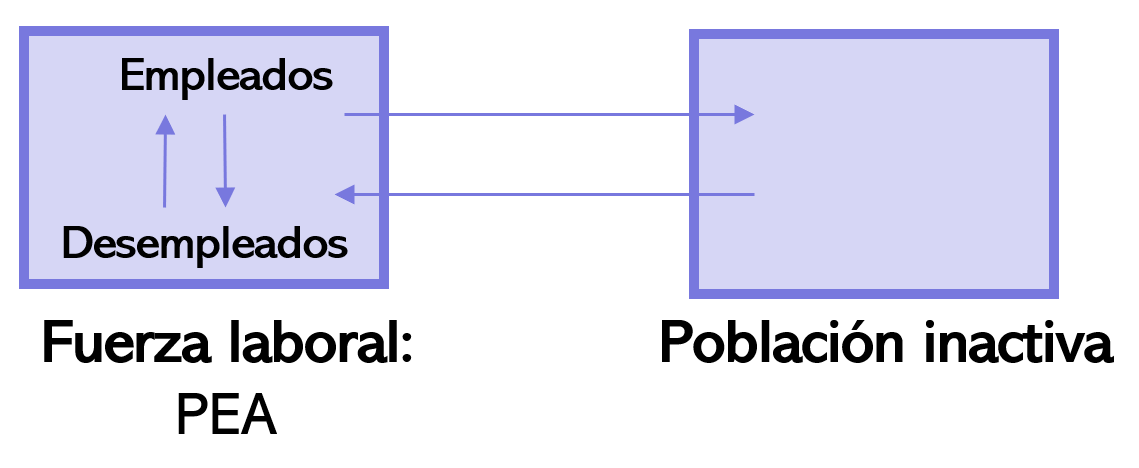
\includegraphics[width=6cm]{Slides Principios de Economia/Figures/P32.png}\
\end{frame}

\begin{frame}{Indicadores básicos del mercado laboral}
\begin{itemize}
    \item Tasa de desempleo: $\frac{\text {Número de desempleados}}{\text{PEA}}$
    \vspace{3mm}
    
        \dangersignw Puede variar por: 
        \begin{itemize}
            \vspace{2mm}
        \item Cambios en el número de desempleados
            \vspace{2mm}
        \item Cambios en la fuerza laboral (PEA)
        \end{itemize}
           \vspace{3mm}
    \item Tasa de empleo: $\frac{\text {Número de empleados}}{\text{Población}}$
    \vspace{3mm}
    \item Tasa de participación: $\frac{\text {PEA}}{\text{Población}}$
\end{itemize}
\end{frame}

\begin{frame}{La tasa de desempleo en Argentina}
\centering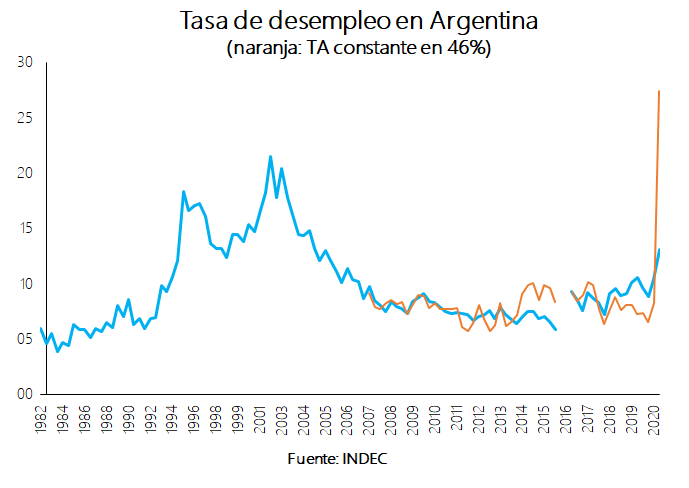
\includegraphics[width=11cm]{Slides Principios de Economia/Figures/P34.png}
\end{frame}

\begin{frame}{Problemas con la serie de desempleo de INDEC}
\centering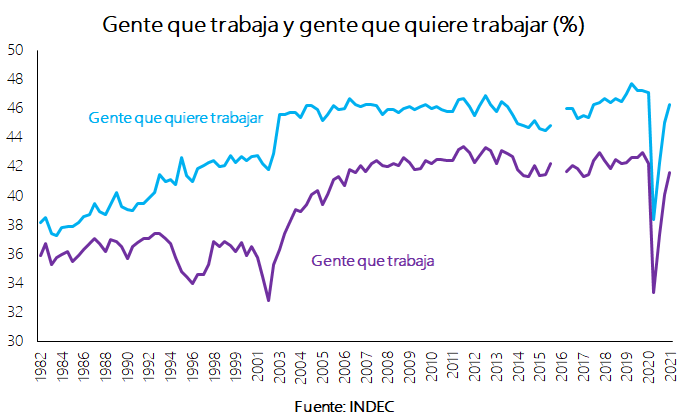
\includegraphics[width=11cm]{Slides Principios de Economia/Figures/C30.15b.png}
\end{frame}

\begin{frame}{El mercado de trabajo en la Argentina (1)}
\centering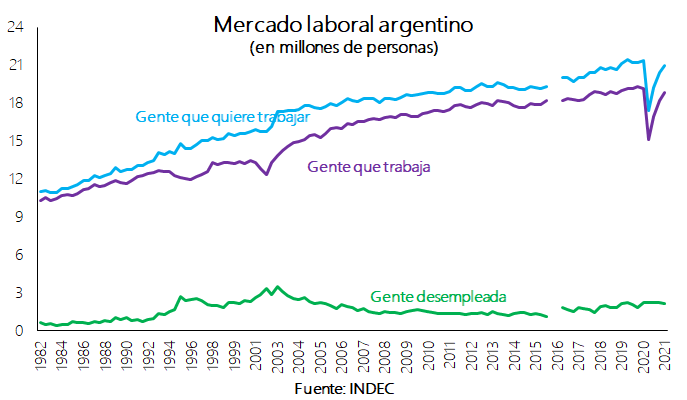
\includegraphics[width=11cm]{Slides Principios de Economia/Figures/C30.16b.png}
\end{frame}

\begin{frame}{El mercado de trabajo en la Argentina (2)}
\centering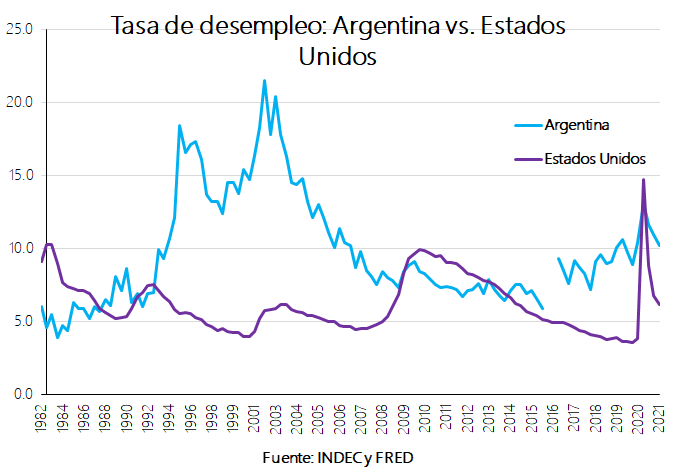
\includegraphics[width=11cm]{Slides Principios de Economia/Figures/C30.17b.png}
\end{frame}

\begin{frame}{La recuperación de EE.UU. tardó en ocupar trabajo}
\centering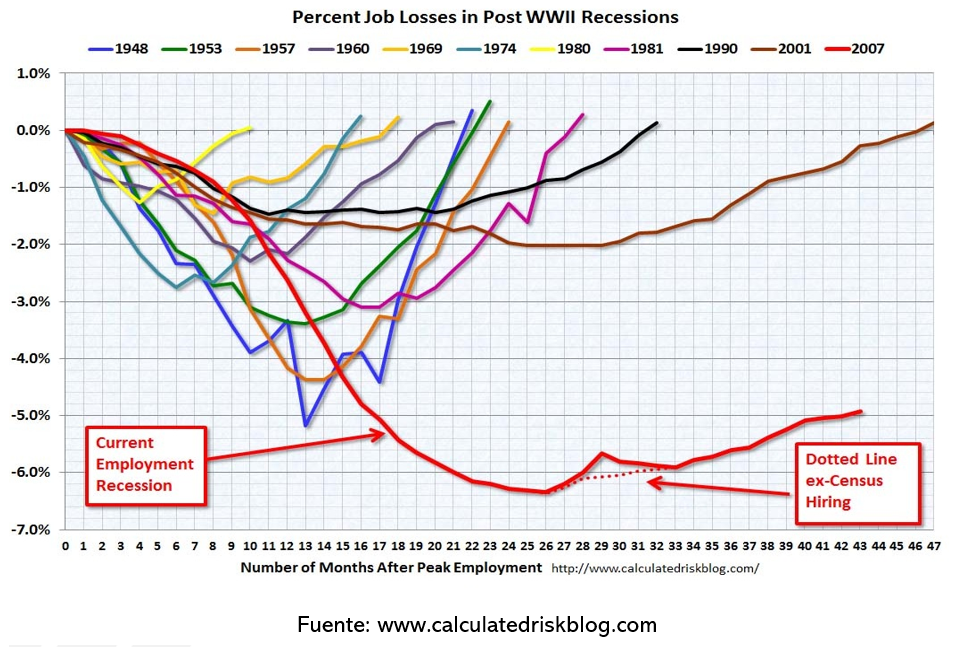
\includegraphics[width=12cm]{Slides Principios de Economia/Figures/P39.png}\
\end{frame}


\begin{frame}{La recuperación de Argentina}
\centering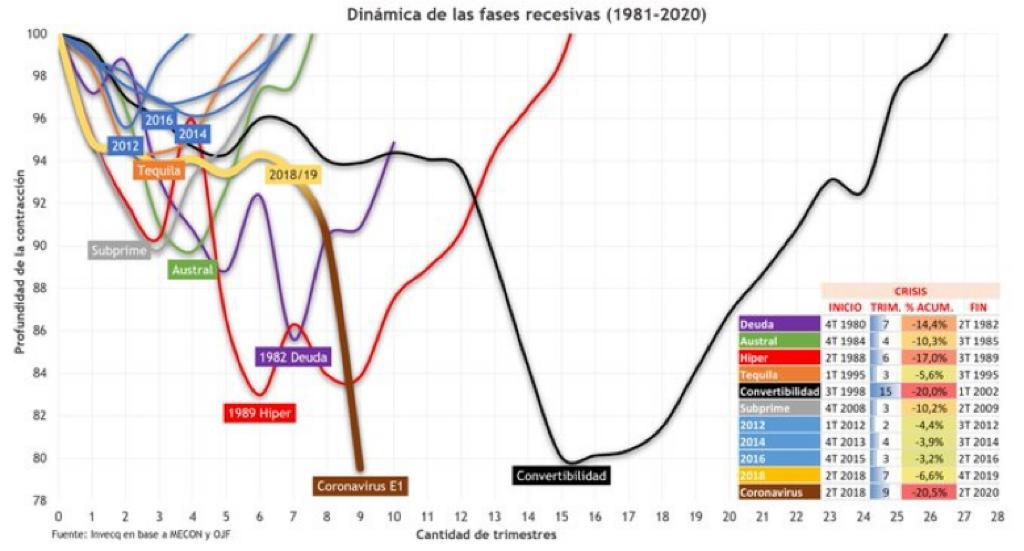
\includegraphics[width=11cm]{Slides Principios de Economia/Recesiones.jpg}\
\end{frame}


\end{document}